\chapter{Design}

The architectural design of MCDTP uses both TCP and UDP connections. Like \cite{Meiss2007}, \cite{He2002}, \cite{Aspera2016}, and \cite{Fan2010}, MCDTP uses the UDP transport protocol for the data transfer and the TCP socket is used for exchanging messages between the server and client. The experimental component of this protocol is the lack of congestion control. As mentioned here, \cite{Aspera2016} \cite{Fan2010}, the observed bottleneck resides on the hosts of an end-to-end transfer. MCDTP seeks to mitigate this through multiple asynchronous data channels and the number of channels is determined when implementing this protocol. A channel acts as a pipe from disk to socket and vice versa. This is how MCDTP tries to provide continuous data flow. As a disclaimer, the term ``packet(s)" hereinafter does not refer to Transport or Network layer packets, the term is used to refer to an Application layer structure used by MCDTP.

\section{Protocol Design}\label{sec:proto-des}

The MCDTP protocol focuses on being a very simple and lean protocol to try and minimize the needed time to process incoming messages or data. The protocol consists of three phases: a two step handshake phase, data transmission phase, and packet retransmission phase. For TCP communication, each packet consists of 15 bytes. Each packet is a header with an optional payload. All headers begin with two fields, ``ptype" and ``subtype". These two fields specify how the packet should be processed. The UDP packet is adjustable in size when implementing MCDTP. It is, however, required to be within the following scope: $13B < size < 64KB$. The 13 byte lower bound is to account for packet header. The 64 kilobyte upper bound can be found here \cite{postel1981ip}. Unlike the TCP packets, UDP packets include payload size with packet size. Since TCP has the option of a payload, when one exists, a second read from the stream will be required to grab the payload. With the UDP packet, it is guaranteed that a packet will be a set size and thus eliminates the need for a second read.

\subsection{Two Step Handshake}

As with many protocols, MCDTP has a handshake step. However, MCDTP performs two handshakes, the first upon connection and the second before a data transfer. The purpose for the two step handshake is for the sake of extensibility, i.e. another step or function could take place between both handshakes.

\subsubsection{Specification Handshake}

The specification handshake occurs when a client connects to the server. Figure \ref{fig:specs} illustrates the type of communication that happens during the handshake.

\begin{figure}[ht]
\centering
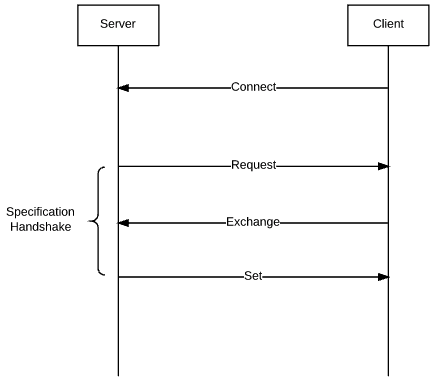
\includegraphics[scale=0.7]{SpecificationHandshake}
\caption{Illustration of Specification Handshake}
\label{fig:specs}
\end{figure}

The purpose of this handshake is ensure that both client and server use the same specifications for a data transfer. These specifications currently include the exchange and selection of ports the client should use for each UDP socket. As a side effect, the server can detect how many data channels the client supports, which is key since not all hosts running MCDTP will be capable of using, or configured to use, the same number of data channels. Thus both hosts need to agree upon how many data channels to use. If one host can support more channels than the other, both hosts will agree to use the smaller of the two. This option is optimal over possible alternatives such as increasing the smaller host to match the larger host, or coercing the transfer to work through mismatching channel count, ``smaller host" refers to the host with the smaller amount of supported channels while ``larger host" refers to the opposite. The aforementioned alternative could work if a host was smaller because it was configured to run conservatively even though the host has the resources to run at a higher performance. However, if the host is smaller because there are fewer resources, then this could potentially cause the host to perform beyond its capacity. Since neither scenario is distinguishable to the client nor server, this option does not work. Coercion could lead to more work needing to be done on the a host depending on which host was larger. Since the concept of a data channel is to pipe file data to network and vice versa, if the client were larger, the server would have to try and multiplex data in a way that the client got roughly equal flow through all channels. If the roles were reversed, the client would need to do additional processing of data to ensure packets were in there appropriate position in file. Ergo, the optimal choice is to simply reduce the larger host to match the smaller host.

\begin{figure}[ht]
\centering
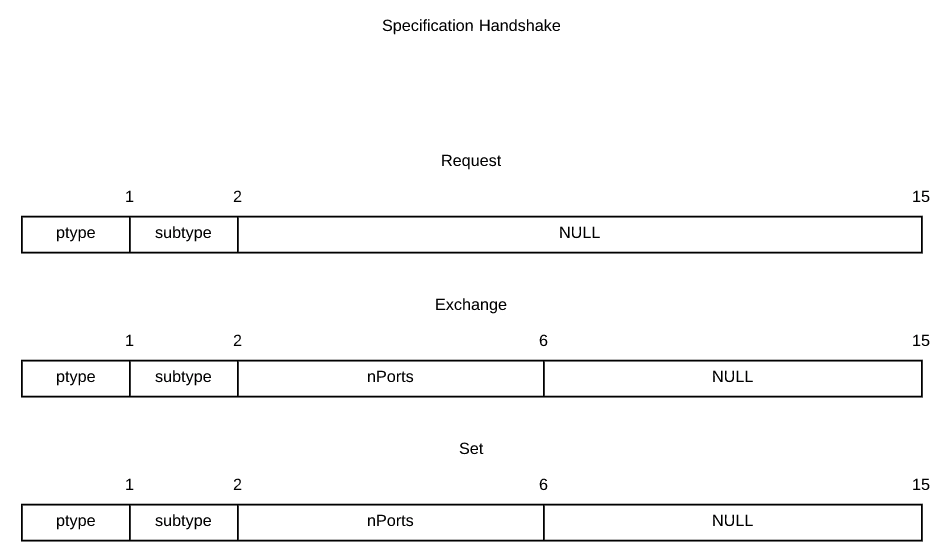
\includegraphics[scale=0.4]{SpecificationHandshakePacketStructures}
\caption{Packet Structure of Specification Handshake}
\label{fig:specs-struct}
\end{figure}

Figure \ref{fig:specs-struct} shows the packet structure of each message, excluding connect, in the handshake. The value of ``ptype" and ``subtype" are as follow for each packet: $Request \rightarrow ptype = \lq{s}\rq,subtype = \lq{r}\rq$, $Exchange \rightarrow ptype = \lq{s}\rq,subtype = \lq{N}\rq$, $Set \rightarrow ptype = \lq{s}\rq,subtype = \lq{n}\rq$. In this handshake, both Exchange and Set have an additional field, ``nPort", and are followed by a payload. The payload consists of port values, which ``nPort" specifies how many port values are in the payload. In order to be as language agnostic as possible, a port is represented as 4 bytes, or a 32bit integer. Given this, the payload size can be calculated so that an exact number of bytes can be read during the second read from stream.

\subsubsection{FTP Handshake}\label{subsec:ftp-hs}

Prior to transferring a file, MCDTP performs another handshake that is similar in design, as can be seen in Figure \ref{fig:ftp-hs}.

\begin{figure}[ht]
\centering
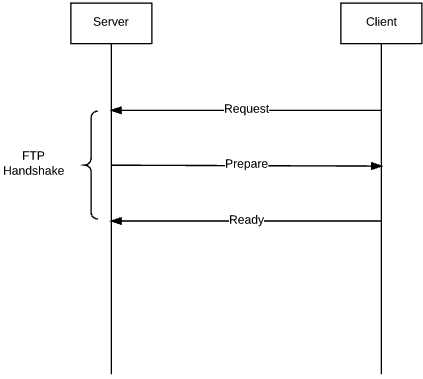
\includegraphics[scale=0.7]{FTPHandshake}
\caption{Illustration of FTP Handshake}
\label{fig:ftp-hs}
\end{figure}

This handshake acts as a concrete step before the data transmission phase and is very simple in design and purpose. This step is so that any asynchronous work that needs to be done first can finish as well as making sure both client and server are prepared for the data transmission phase, which is more of an implementation discussion and will be further discussed in chapter \ref{chp:impl}. Figure \ref{fig:ftp-struct} is an illustration of the structure of each message in the handshake.

\begin{figure}[ht]
\centering
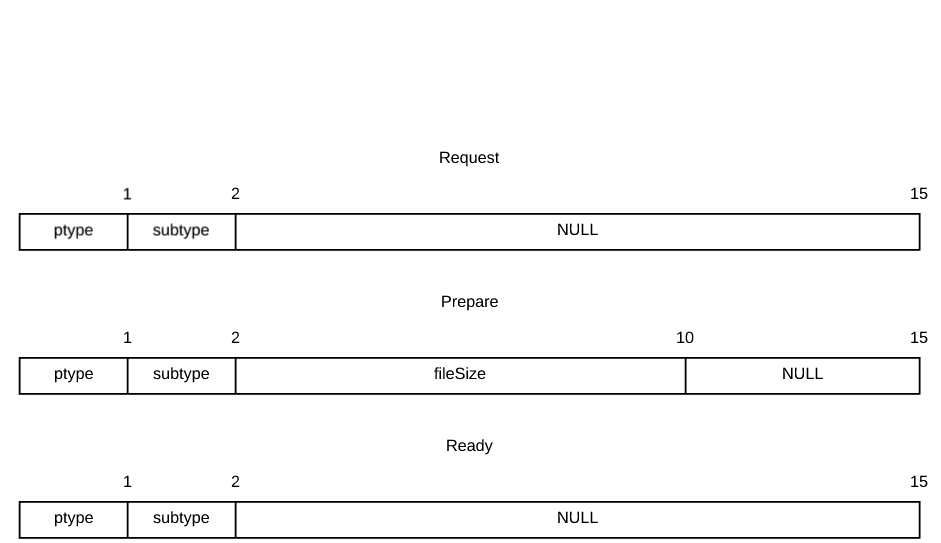
\includegraphics[scale=0.4]{FTPHandshakePacketStructures}
\caption{Packet Structure of FTP Handshake}
\label{fig:ftp-struct}
\end{figure}

 The value of ``ptype" and ``subtype" are as follow for each packet: $Request \rightarrow ptype = \lq{t}\rq,subtype = \lq{r}\rq$, $Prepare \rightarrow ptype = \lq{t}\rq,subtype = \lq{p}\rq$, $Ready \rightarrow ptype = \lq{t}\rq,subtype = \lq{R}\rq$. The only information exchanged in this handshake is the size of the file that will be transferred, from server to client. Note that handling file selection has been omitted and will be further discussed in chapter \ref{chp:c-fw}. Once the client is prepared for transfer and has signaled the server that it is ready, both hosts begin the data transmission phase of the MCDTP protocol.

\subsection{Data Transmission}

The data transmission phase is the second phase in the MCDTP protocol and is comprised mostly of the transmission of a file using the data channels setup in phase 1. The upper portion of Figure \ref{fig:data-tr} illustrates the communication between server and client. The large arrow from server to client at the top represents the data flow for a single channel. The blue in this representation symbolizes the transmission of the file. The packet retransmission phase and this phase have slight overlap, which is further discussed in section \ref{subsec:pack-retr}.

\begin{figure}[ht]
\centering
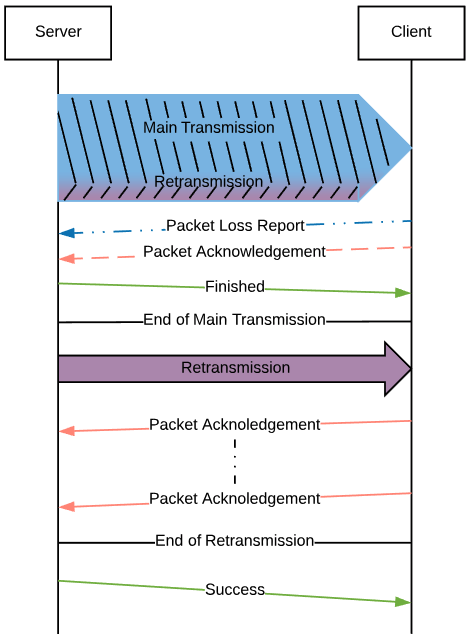
\includegraphics[scale=0.5]{DataTransfer}
\caption{Illustration of Data Transfer}
\label{fig:data-tr}
\end{figure}

The packet structure of the data transmitted over each channel is shown in Figure \ref{fig:data-tr-struct}. Note that the packet size is not definitively set. As stated above, the packet size can range from $13B < size < 64KB$ and is something that needs to be set at an implementation level. The ``seqNum" field is the position in file that the data should be written to. To maintain packet size, ``dLen" is used to determine exactly how much of ``data" is meaningful to the transfer. The ``flag" field acts as a control flag. When $flag=0$, the packet is a regular packet. A retransmitted packet has a ``flag" value of 1 and 2 is to signal to the client that the channel is switching to the packet retransmission phase. The final packet is illustrated by the green communication line labeled ``Finished" in Figure \ref{fig:data-tr}, which is sent over the UDP channel.

\begin{figure}[ht]
\centering
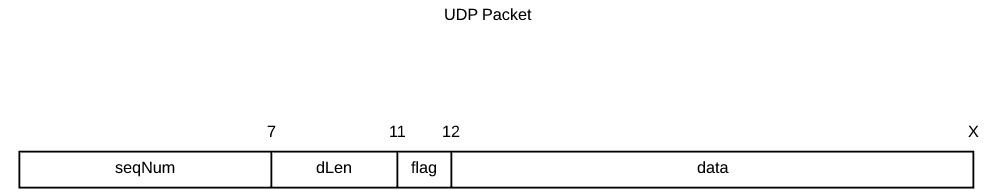
\includegraphics[scale=0.4]{DataTransferPacketStructure}
\caption{Packet Structure of Data Transfer}
\label{fig:data-tr-struct}
\end{figure}

As previously mentioned, MCDTP is an experimental protocol. The experimental component attempts to perform a file transfer without the use of congestion control. The protocol tries to exploit the common operating system behavior that when a socket is created, it is given its own receive buffer. With each channel getting its own receive buffer, there is more space to hold incoming packets giving opportunity for handling more data at the Application layer.

\subsection{Packet Retransmission}\label{subsec:pack-retr}

The packet retransmission phase is capable of starting during the data transmission phase. The purpose of this is to hopefully recover packets along the way to minimize the duration of this phase and ultimately achieve a successful transfer faster. As can be seen in Figure \ref{fig:data-tr}, retransmission consumes a very small portion of bandwidth so as not to impede upon the main transmission during the data transmission phase. The dashed communication lines labeled ``Packet Loss Report" and ``Packet Acknowledgement", which share the same structure as is evident in Figure \ref{fig:pack-rec-struct}, only occur when packet loss or packet recovery is detected and are sent over the TCP socket. The values for ``ptype" and ``subtype" are as follows: $Packet Loss Report \rightarrow ptype = \lq{t}\rq,subtype = \lq{l}\rq$ and $Packet Acknowledgement \rightarrow ptype = \lq{t}\rq,subtype = \lq{a}\rq$. The ``seqNum" field identifies the UDP packet the message is about and the ``port" field identifies which channel the UDP packet belongs to.

\begin{figure}[ht]
\centering
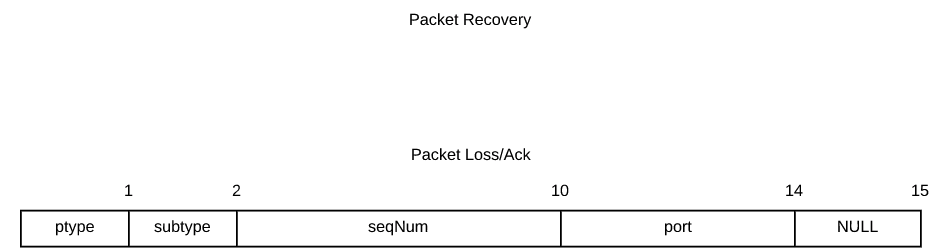
\includegraphics[scale=0.4]{PacketRecoveryStructure}
\caption{Packet Loss and Ack Report Structure}
\label{fig:pack-rec-struct}
\end{figure}

After the data transmission phase finishes, the packet retransmission phase is able to consume more bandwidth. The ``Finished" packet is also placed in recovery to ensure the client receives this. Once the client sends an acknowledgement for this packet, that channel will be in the packet retransmission phase on both the client and server, which is represented by the middle segment of Figure \ref{fig:data-tr}.

\begin{figure}[ht]
\centering
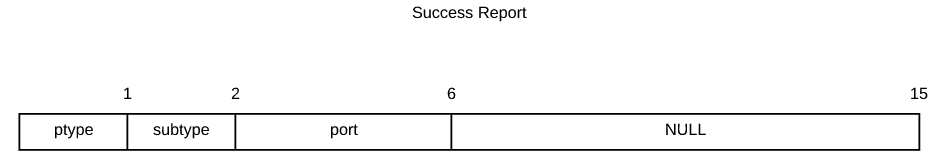
\includegraphics[scale=0.4]{SuccessPacketStructure}
\caption{Packet Structure of Success Report}
\label{fig:success-struct}
\end{figure}

Like RBUDP \cite{He2002}, a channel will continue this phase until the server has received an acknowledgement for all packets that are in recovery for that channel. Once all packets have made it, the server sends a success report, Figure \ref{fig:success-struct}, over TCP thus concluding the work the channel specified by the ``port" field. The ``ptype" and ``subtype" are set to $`t'$ and $`S'$, respectively. One all channels have succeeded, the session between the client and server is concluded.